\chapter{Design and Implementation}
\label{sec:design}

As mentioned previously, we expect NVBM to be exposed across a memory bus and
not via a legacy disk interface.  In addition to the file system and block
device overhead measured in Chapter~\ref{sec:fs}, using the PCI interface
(256~ns latency~\citep{Holden06}) or even a kernel-based syscall API (89.2 and
76.4~ns for POSIX \texttt{read/write}) would add significant overhead to NVBM's
access latencies (50--150~ns).  As shown in Chapter~\ref{sec:fs}, the overhead
of using file systems or buffered updates would also be prohibitively large.
Further, given the performance and energy cost of moving data, we believe that
all data should reside in a single-level store where no distinction is made
between volatile and persistent storage and all updates are performed in-place.
We therefore propose that data access should use userspace libraries and APIs
that map data into the process's address space.

However, the same properties that allow systems to take full advantage
of NVBM's performance properties also introduce challenges.  In
particular, one of the biggest obstacles is that current processors do
not provide primitives to order memory writes.  Combined with the fact
that the memory controller can reorder writes (at a cache line
granularity), current mechanisms for updating data structures are
likely to cause corruption in the face of power or software failures.
For example, assume that a hash table insert requires the write of a
new hash table object and is followed by a pointer write linking the
new object to the hash table.  A reordered write could propagate the
pointer to main memory before the object and a failure at this stage
would cause the pointer to link to an undefined memory region.
Processor modifications for ordering can be complex~\citep{Condit09},
do not show up on vendor roadmaps, and will likely be preceded by NVBM
availability.

To address these issues, our design and implementation focuses on
three different layers. First, in Chapter~\ref{sec:flush}, we describe
how we implement ordering and flushing of data on existing processors.
However, this low-level primitive is not sufficient for atomic updates
larger than 8~bytes.  In addition, we therefore also require 
versioning CDDSs, whose design principles are described in
Chapter~\ref{sec:cdds_overview}.  After discussing our CDDS B-Tree
implementation in Chapter~\ref{sec:cdds_btree} and some of the open
opportunities and challenges with CDDS data structures in
Chapter~\ref{sec:cdds_discuss}, Chapter~\ref{sec:kv} describes Tembo,
the system resulting from the integration of our CDDS B-Tree into a
distributed Key-Value system.

\section{Flushing Data on Current Processors}
\label{sec:flush}

As mentioned earlier, today's processors have no mechanism for
preventing memory writes from reaching memory and doing so for
arbitrarily large updates would be infeasible.  Similarly, there is no
guarantee that writes will not be reordered by either the processor or
by the memory controller.  While processors support a \texttt{mfence}
instruction, it only provides write visibility and does not guarantee
that all memory writes are propagated to memory (NVBM in this case) or
that the ordering of writes is maintained.  While cache contents can
be flushed using the \texttt{wbinvd} instruction, it is a
high-overhead operation (multiple ms per invocation) and flushes the
instruction cache and other unrelated cached data.  While it is
possible to mark specific memory regions as write-through, this impacts
write throughput as all stores have to wait for the data to reach main
memory.


To address this problem, we use a combination of tracking recently
written data and use of the \texttt{mfence} and \texttt{clflush}
instructions.  \texttt{clflush} is an instruction that invalidates the
cache line containing a given memory address from all levels of the
cache hierarchy, across multiple processors.  If the cache line is dirty
(i.e., it has uncommitted data), it is written to memory before
invalidation. The \texttt{clflush} instruction is also ordered by the
\texttt{mfence} instruction.
%\footnote{Instructions available on Intel and AMD CPUs since 2000 and 2003.}
Therefore, to commit a series of memory writes, we first execute an
\texttt{mfence} as a barrier to them, execute a \texttt{clflush} on
every cacheline of all modified memory regions that need to be
committed to persistent memory, and then execute another
\texttt{mfence}.  In this paper, we refer to this instruction
sequence as a \textit{\texttt{flush}}.  As microbenchmarks in
Chapter~\ref{sec:flush_perf} show, using \texttt{flush} will be
acceptable for most workloads.

While this description and tracking dirty memory might seem complex,
this was easy to implement in practice and can be abstracted away by
macros or helper functions.  In particular, for data structures, all
updates occur behind an API and therefore the process of
\texttt{flush}ing data to non-volatile memory is hidden from the
programmer. Using the simplified hash table example described above,
the implementation would first write the object and \texttt{flush}
it. Only after this would it write the pointer value and then
\texttt{flush} again.  This two-step process is transparent to the
user as it occurs inside the insert method.

Finally, one should note that while \texttt{flush} is necessary for
durability and consistency, it is not sufficient by itself.  If any
metadata update (e.g., rebalancing a tree) requires an atomic update
greater than the 8~byte atomic write provided by the hardware, a
failure could leave it in an inconsistent state.  We therefore need
the versioning approach described below in Chapters~\ref{sec:cdds_overview}
and~\ref{sec:cdds_btree}.

\section{CDDS Overview}
\label{sec:cdds_overview}

Given the challenges highlighted at the beginning of
Chapter~\ref{sec:design}, an ideal data store for non-volatile memory
must have the following properties:

\begin{smitemize}
\item \textbf{Durable}: The data store should be durable.  A fail-stop
  failure should not lose committed data.

\item \textbf{Consistent}: The data store should remain consistent
  after every update operation. If a failure occurs during an update,
  the data store must be restored to a consistent state before further
  updates are applied.

\item \textbf{Scalable}: The data store should scale to
  arbitrarily-large sizes.  When compared to traditional data stores,
  any space, performance, or complexity overhead should be minimal.

\item \textbf{Easy-to-Program}: Using the data store should not
  introduce undue complexity for programmers or unreasonable
  limitations to its use.

\end{smitemize}


\begin{figure*}[tbh]
\centerline{
\begin{tikzpicture}[scale=0.75, transform shape]
\begin{scope}
[level 1/.style={sibling distance=8.5cm},
 level 2/.style={sibling distance=3.3cm}]
[node distance=2cm on grid, >=stealth', auto]
 \node[nd={d,l,l}] {
    \btnode{text}{99}{1}{6}
    \btnode{second}{99}{6}{-}
 }
 child {node[nd={d,d,d}] (b1) {
    \btnode{text}{20}{4}{6}
    \btnode{second}{99}{1}{4}
    \btnode{third}{99}{4}{6}
   }
   child{node[nd={d,d,d}] (c2) {
       \btnode{text}{5}{4}{6}
       \btnode{second}{10}{5}{6}
       \btnode{third}{20}{4}{6}
       }
   }
   child{node[nd={d,d,d}] (c1) {
       \btnode{text}{5}{2}{4}
       \btnode{second}{20}{3}{4}
       \btnode{third}{99}{1}{4}
       }
   }
   child{node[nd={l,l,l}] (c3) {
       \btnode{text}{40}{4}{-}
       \btnode{second}{99}{4}{-}
       }
   }
 }
 child [parent anchor = south] {node[nd={l,l,l}] (b2) {
    \btnode{text}{10}{6}{-}
    \btnode{second}{20}{6}{-}
    \btnode{third}{99}{6}{-}
   } 
   child [parent anchor = one south] {node[nd={l,l,l}] {
       \btnode{text}{5}{6}{-}
       \btnode{second}{8}{7}{-}
       \btnode{third}{10}{6}{-}
     }
   }
   child [parent anchor = south]{node[nd={l,d,l}] {
       \btnode{text}{13}{9}{-}
       \btnode{second}{15}{6}{8}
       \btnode{third}{20}{6}{-}
     }
   }
 };
 \draw [-] (b2.three south) to  (c3.north); 
\end{scope}
\begin{scope}[xshift=9cm, yshift=-1.75cm, node distance=4mm]
\node (live) [rectangle, thick, draw=black!75, inner sep=4mm, 
              label=right:Live entry] {\\};
\node (dead) [below =of live, thick, draw=black!75, fill=black!25,
              inner sep=4mm, label=right:Dead entry] {\\};
\end{scope}
\begin{scope}[xshift=9.5cm]
\node [rectangle, thick, draw=black!75, inner sep=1mm,% font=\large,
       align=center]{
{\small $Key$}\\
$\left[ {Start \atop Version} , {End \atop Version} \right)$
%% $
%% \left( \begin{array}{c@{,}c}
%% Start & End \\
%% Version & Version
%% \end{array}
%% \right)
%% $
%% \begin{tabular}{cc}
%%   \multicolumn{2}{c}{Key} \\
%%   Start & End \\
%%   Version & Version
%% \end{tabular}
};
%       align=center]{ Key \\ $[$start, end$)$ };
\end{scope}
\end{tikzpicture}
}
%\vspace{-0.1in}
\caption{Example of a CDDS B-Tree}
\label{fig:cd-btree}
%\vspace{-0.15in}
\end{figure*}

We believe it is possible to meet the above properties by storing data
in Consistent and Durable Data Structures (CDDSs), i.e., hardened
versions of conventional data structures currently used with volatile
memory.  The ideas used in constructing a CDDS are applicable to a
wide variety of linked data structures and, in this paper, we
implement a CDDS B-Tree because of its non-trivial implementation
complexity and widespread use in storage systems.  We would like to
note that the design and implementation of a CDDS only addresses
\textit{physical} consistency, i.e., ensuring that the data structure
is readable and never left in a corrupt state.  Higher-level layers
control \textit{logical} consistency, i.e., ensuring that the data
stored in the data structure is valid and matches external integrity
constraints.  Similarly, while our current system implements a simple
concurrency control scheme, we do not mandate concurrency control to
provide isolation as it might be more efficient to do it at a higher
layer.

A CDDS is built by maintaining a limited number of versions of the
data structure with the constraint that an update should not weaken
the structural integrity of an older version and that updates are
atomic.  This versioning scheme allows a CDDS to provide consistency
without the additional overhead of logging or shadowing.  A CDDS thus
provides a guarantee that a failure between operations will never
leave the data in an inconsistent state.  As a CDDS never acknowledges
completion of an update without safely committing it to non-volatile
memory, it also ensures that there is no silent data loss.



\section{Versioning for Durability}
\label{sec:versioning_overview}

Internally, a CDDS maintains the following properties:

\begin{smitemize}
  \item There exists a version number for the most recent consistent
    version.  This is used by any thread which wishes to read from the
    data structure.
  \item Every update to the data structure results in the creation of
    a new version.
  \item During the update operation, modifications ensure that existing 
    data contained in older versions is never overwritten. Such
    modifications are performed by either using atomic operations
    or copy-on-write style changes.
  \item After all the modifications for an update have been made
    persistent, the most recent consistent version number is updated
    atomically and the operation is committed .
\end{smitemize}


\subsection{Garbage Collection}

Along with support for multiple versions, a CDDS also tracks versions
of the data structure that are being accessed.  Knowing the oldest
version which has a non-zero reference count has two benefits.  First,
we can garbage collect older versions of the data structure. Garbage
collection (GC) is run in the background and helps bound the space
utilized by eliminating data that will not be referenced in the
future.  Second, knowing the oldest active version can also improve
performance by enabling intelligent space reuse in a CDDS\@. When
creating a new entry, the CDDS can proactively reclaim the space used
by older inactive versions.



\subsection{Failure Recovery}

Insert or delete operations may be interrupted due to operating system
crashes or power failures.  By definition, the most recent consistent
version of the data structure should be accessible on recovery.
However, an in-progress update needs to be removed as it belongs to an
uncommitted version.  We handle failures in a CDDS by using a `forward
garbage collection' procedure during recovery.  This process involves
discarding all update operations which were executed after the most
recent consistent version.  Newly created entries can be discarded while
older entries with in-progress update operations are reverted.

% The recovery procedure is closely related to the
% concurrency model used. The currently implemented shared reader,
% single writer concurrency model enables fast and simple recovery.

%\begin{figure*}[tbh]
%  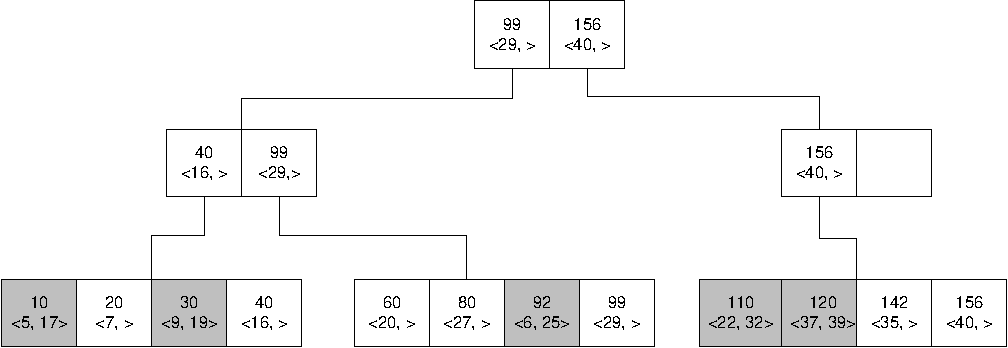
\includegraphics[width=\textwidth]{figs/cd-btree}
%  \caption{Example of a Consistent and Durable B-Tree}
%  \label{fig:cd-btree} 
%\end{figure*}


\section{CDDS B-Trees}
\label{sec:cdds_btree}

As an example of a CDDS, we selected the B-Tree~\citep{Comer79} data
structure because of its widespread use in databases, file systems,
and storage systems.  This section discusses the design and
implementation of a consistent and durable version of a B-Tree.  Our
B-Tree modifications\footnote{In reality, our B-Tree is a B+~Tree with
  values only stored in leaves.} have been heavily inspired by
previous work on multi-version data
structures~\citep{Becker96,Varman97}.  However, our focus on
durability required changes to the design and impacted our
implementation.  We also do not retain all previous versions of the
data structure and can therefore optimize updates.

In a CDDS B-Tree node, shown in Figure~\ref{fig:cd-btree}, the key and
value stored in a B-Tree entry is augmented with a start and end
version number, represented by unsigned 64-bit integers.  A B-Tree
node is considered `live' if it has at least one live entry.  In turn,
an entry is considered `live' if it does not have an end version
(displayed as a `$-$' in Figure~\ref{fig:cd-btree}). To bound space utilization, in
addition to ensuring that a minimum number of entries in a B-Tree node
are used, we also bound the minimum number
of live entries in each node.  Thus, while the CDDS B-Tree API is
identical to normal B-Trees, the implementation differs
significantly.
In the rest of this section, we use the \textit{lookup},
\textit{insert}, and \textit{delete} operations to illustrate how the
CDDS B-Tree design guarantees consistency and durability.
%\footnote{A longer
%  technical report~\citep{Venkataraman10} presents more
%  details on all CDDS B-Tree operations and their corresponding
%  implementations.}.


\subsection{Lookup}
\label{sec:btree_lookup}

We first briefly describe the lookup algorithm, shown in 
Algorithm~\ref{alg:btree_lookup}.  For ease of explanation,
the pseudocode in this and following algorithms does not
include all of the design details.  The algorithm uses the
\texttt{find} function to recurse down the tree
(lines~\ref{line:l_descend}--\ref{line:l_descend_done}) until it finds
the leaf node with the correct key and value.

\begin{algorithm}[t]
\dontprintsemicolon
\linesnumbered

\SetAlFnt{\sf}
\SetAlCapFnt{\sf}

\SetKwFunction{GetLastConsistentVersion}{get\_last\_consistent\_version}
\SetKwFunction{GetNumEntries}{get\_num\_entries}
\SetKwFunction{NumLiveEntries}{num\_live\_entries}
\SetKwFunction{Insert}{insert}
\SetKwFunction{IsInnerNode}{is\_inner\_node}
\SetKwFunction{Lookup}{lookup}
\SetKwFunction{Find}{find}

\KwIn{k: key, r: root}
\KwOut{val: value}
\Begin(\Lookup{k, r}){
    $v \leftarrow  current\_version$\; \nllabel{line:l_version}
    $n \leftarrow r$\;
    \While { \IsInnerNode{n} } {  \nllabel{line:l_descend}
      $entry\_num \leftarrow \Find{k, n, v}$\; 
      $n \leftarrow n[entry\_num].child$\; \nllabel{line:l_descend_done}
    }
    $entry\_num \leftarrow \Find{k, n, v}$\; 
    \Return{$n[entry\_num].value$}\;
}
\BlankLine
\Begin(\Find{k, n, v}) {
  $l \leftarrow 0$\;
  $h \leftarrow \GetNumEntries{n}$\;
  \While(\tcp*[f]{Binary Serch}) { $l < h$ } { \nllabel{line:l_binary}
    $m \leftarrow (l + h)/2$\;
    \If { $k \leq n[m].key$ } {
      $h \leftarrow m-1$\;
    } \lElse $l \leftarrow m+1$\;   \nllabel{line:l_binary_done}
  }
  \While { $h < \GetNumEntries {n}$ } { \nllabel{line:vcheck}
    \If { $n[h].start \leq v$ } {
      \If { $n[h].end > v \quad \| \quad n[h].end = 0$ } {
        $break$\;
      }
    }
    $h \leftarrow h+1$\;  \nllabel{line:vcheck_done}
  }
  \Return{$h$}\;
}
\caption{CDDS B-Tree Lookup}
\label{alg:btree_lookup}
\end{algorithm}


Consider a lookup for the key $10$ in the CDDS B-Tree shown in
Figure~\ref{fig:cd-btree}.  After determining the most current version
(version $9$, line~\ref{line:l_version}), we start from the root node
and pick the rightmost entry with key $99$ as it is the next largest
valid key.  Similarly in the next level, we follow the link from the
leftmost entry and finally retrieve the value for $10$ from the leaf
node.

Our implementation currently optimizes lookup performance by ordering
node entries by key first and then by the start version number.
This involves extra writes during inserts to shift entries but
improves read performance by enabling a binary search within nodes
(lines~\ref{line:l_binary}--\ref{line:l_binary_done} in
\texttt{find}).  While we have an alternate implementation that
optimizes writes by not ordering keys at the cost of higher lookup
latencies, we do not use it as our target workloads are
read-intensive.  Finally, once we detect the right index in the node,
we ensure that we are returning a version that was valid for $v$, the
requested version number
(lines~\ref{line:vcheck}--\ref{line:vcheck_done}).


\begin{algorithm}[t]
\dontprintsemicolon
\linesnumbered

\SetAlFnt{\sf}
\SetAlCapFnt{\sf}

\SetKwFunction{GetLastConsistentVersion}{get\_last\_consistent\_version}
\SetKwFunction{GetNumEntries}{get\_num\_entries}
\SetKwFunction{SetNumEntries}{set\_num\_entries}
\SetKwFunction{CanReuseVersion}{can\_reuse\_version}
\SetKwFunction{SplitInsert}{split\_insert}
\SetKwFunction{Flush}{flush}
\SetKwFunction{InsertKey}{insert\_key}
\SetKwFunction{NumLiveEntries}{num\_live\_entries}
\SetKwFunction{MinLiveEntries}{min\_live\_entries}
\SetKwFunction{Insert}{insert}
\SetKwFunction{NewNode}{new\_node}

\KwIn{k: key, r: root}
\Begin(\InsertKey{k, r}){
    $v \leftarrow current\_version$\; \nllabel{line:i_version1}
    $v'\leftarrow v+1$\; \nllabel{line:i_version2}
    \tcp{Recurse to leaf node (n)}\;
    %\vdots\;
    %\BlankLine
    $y \leftarrow \GetNumEntries{n} $\;
    \If(\tcp*[f]{Node Full}){$y = node\_size$} {  \nllabel{line:i_full}
      \If {entry\_num = \CanReuseVersion{$n, y$}}{
        \tcp{ Remove the oldest entry }
        %      (again maintaining sorted order)
        % \BlankLine
        % \tcp{ Insert in sorted order} 
        $n[entry\_num].key \leftarrow k $\;
        $n[entry\_num].start \leftarrow v' $\;
        $n[entry\_num].end \leftarrow 0 $\;
        \Flush{$n[entry\_num]$} \; \nllabel{line:i_nslot_flush}\;
      }
      \Else {
        \SplitInsert{$n$, $k$, $v'$}\;
        %\BlankLine
        \tcp{Update inner nodes}\;
      }
    }
    \Else{
      $n[y].key \leftarrow k $\;
      $n[y].start \leftarrow v' $\;
      $n[y].end \leftarrow 0 $\;
      \Flush{$n[y]$} \; \nllabel{line:i_ny_flush}\;
    }
%   XXX - Too confusing. What about split nodes? In that case n is
%   invalid.
%    \SetNumEntries{$n$, $y+1$}\;
    $current\_version \leftarrow v'$\; \nllabel{line:i_upv}
    \Flush{$current\_version$}\;       \nllabel{line:i_flush_version}
}
\BlankLine
\Begin(\CanReuseVersion{n, y}){
    $cv \leftarrow \GetLastConsistentVersion$ \;
    $entry\_num \leftarrow 0$ \;
    \For {$i = 1$ to $y$} { 
        \If{$n[i].end > 0$ and $n[i].end < cv$} { \nllabel{line:i_reuse}
           \If{$entry\_num = 0$ or $i < entry\_num$} { 
             $entry\_num = i$ \;
            }
        }
    }
    \Return $entry\_num$ \;
}
\caption{CDDS B-Tree Insertion}
\label{alg:btree_insert}
\end{algorithm}

\begin{algorithm}[t]
\dontprintsemicolon
\linesnumbered

\SetAlFnt{\sf}
\SetAlCapFnt{\sf}

\SetKwFunction{GetLastConsistentVersion}{get\_last\_consistent\_version}
\SetKwFunction{GetNumEntries}{get\_num\_entries}
\SetKwFunction{SetNumEntries}{set\_num\_entries}
\SetKwFunction{SplitInsert}{split\_insert}
\SetKwFunction{Flush}{flush}
\SetKwFunction{InsertKey}{insert\_key}
\SetKwFunction{NumLiveEntries}{num\_live\_entries}
\SetKwFunction{MinLiveEntries}{min\_live\_entries}
\SetKwFunction{Insert}{insert}
\SetKwFunction{NewNode}{new\_node}
\KwIn{n: node, k: key, version: v}
\Begin(\SplitInsert{n, k, v}){
    $l \leftarrow \NumLiveEntries{n} $\;
    $m_{l} \leftarrow \MinLiveEntries $\;
    \If {$l > 4*m_{l}$}{
      $nn_{1} \leftarrow \NewNode $\;
      $nn_{2} \leftarrow \NewNode $\;
      \For {$i = 1$ to $l/2 $} { 
        \Insert{$nn_{1}, n[i].key, v$}
      }
      \For {$i = l/2 + 1$ to $l$} {
        \Insert{$nn_{2}, n[i].key, v$}
      }
      \If {$k < n[l/2].key$} {
        \Insert{$nn_{1}, k, v$}
      } 
      \lElse { 
        \Insert{$nn_{2}, k, v$} \;
      }
      \Flush{$nn_{1}, nn_{2}$} \; \nllabel{line:i_flush_nn1_nn2}
    }
    \Else {
      $nn \leftarrow \NewNode $\;
      \For {$i = 1$ to $l$} { 
        \Insert{$nn, n[i].key, v$}
      }
      \Insert{$nn, k, v$} \;
      \Flush{$nn$} \; \nllabel{line:i_flush_nn}
    }
    \For {$i = 1$ to $l$} { \nllabel{line:i_endversion}
      $n[i].end \leftarrow v $\; \nllabel{line:i_endversion_end}
    }
    \Flush{$n$} \;
}
\caption{CDDS B-Tree Split-Insert}
\label{alg:btree_split_insert}
\end{algorithm}


\begin{comment}

\begin{figure*}[tbh]
\begin{tikzpicture}
[level 1/.style={sibling distance=3.3cm}]
[node distance=2cm on grid, >=stealth', auto]
 \node[nd={l,d,l}] {
    \btnode{text}{20}{4}{-}
    \btnode{second}{99}{1}{4}
    \btnode{third}{99}{4}{-}
 }
 child {node[nd={l,l,l}] (b2) {
    \btnode{text}{5}{4}{-}
    \btnode{second}{10}{5}{-}
    \btnode{third}{20}{4}{-}
   } 
 }
 child {node[nd={d,d,d}] (b1) {
    \btnode{text}{5}{2}{4}
    \btnode{second}{20}{3}{4}
    \btnode{third}{99}{1}{4}
   }
 }
 child {node[nd={l,l,l}] (b3) {
    \btnode{text}{40}{4}{-}
    \btnode{second}{99}{4}{-}
   }
 };
\end{tikzpicture}
\caption{Example of a consistent, durable B-Tree, for lookup}
\label{fig:l-cd-btree}
\end{figure*}

\end{comment}



\subsection{Insertion}
\label{sec:btree_insert}

The algorithm for inserting a key into a CDDS B-Tree is shown in
Algorithm~\ref{alg:btree_insert}. Our implementation of the algorithm
uses the \texttt{flush} operation (described in Chapter~\ref{sec:flush}) 
to perform atomic operations on a cacheline. Consider the case where a 
key, $12$, is inserted into the B-Tree shown in Figure~\ref{fig:cd-btree}. 
First, an algorithm similar to lookup is used to find the leaf node that
contains the key range that $12$ belongs to. In this case, the
right-most leaf node is selected. As shown in
lines~\ref{line:i_version1}--\ref{line:i_version2}, the current
consistent version is read and a new version number is generated. As
the leaf node is full, we first use the \texttt{can\_reuse\_version}
function to check if an existing dead entry can be reused.  As shown
in line~\ref{line:i_reuse}, an entry can be reused if its end
version is older than the current consistent version. In this
case, the entry with key $15$ died at version $8$ and is reused.
To reuse a slot we first remove the key from the node and shift the
entries to maintain them in sorted order. Now we insert the new key
and again shift entries as required. For each key shift, we ensure 
that the data is first \texttt{flush}ed to another slot before it is 
overwritten. This ensures that the safety properties specified in
Chapter~\ref{sec:versioning_overview} are not violated.
While not described in the algorithm, if an empty entry was detected
in the node, it would be used and the order of the keys,
as specified in Chapter~\ref{sec:btree_lookup}, would be maintained.  

%This step also \texttt{flush}es updated entries in order such that safety
%properties specified in Chapter~\ref{sec:versioning_overview} are
%never violated.


%Another example of space reuse is shown in Figure~\ref{fig:reuse-ver}. 
%\begin{figure}[htb]
%  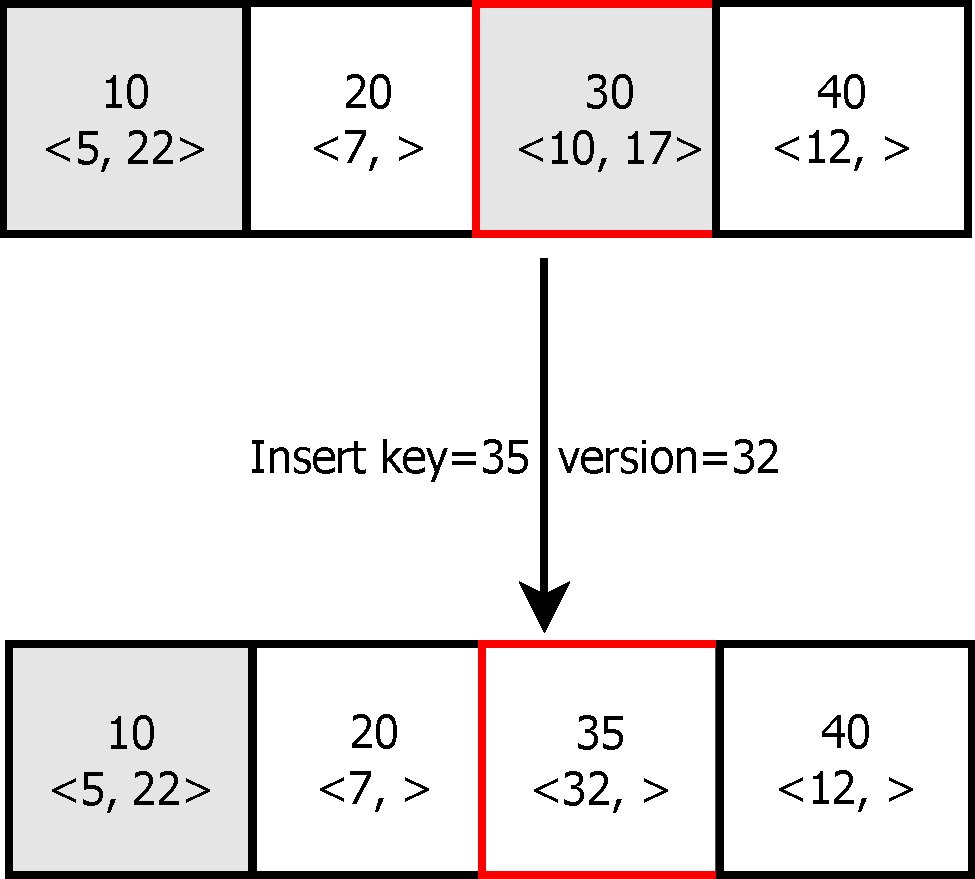
\includegraphics[width=\columnwidth]{figs/version_stealing}
%  \caption{Example of space reuse in a B-Tree leaf}
%  \label{fig:reuse-ver} 
%\end{figure}

If no free or dead entry was found, a \texttt{split\_insert}, similar
to a traditional B-Tree split, would be performed. \texttt{split\_insert},
shown in Algorithm~\ref{alg:btree_split_insert}, is a copy-on-write style
operation in which existing entries are copied before making a
modification. As an example, consider the node shown in 
Figure~\ref{fig:split_example}, where the key $40$ is being inserted.  
We only need to preserve the `live' entries for further updates and 
\texttt{split\_insert} creates one or two new nodes based on the number
of live entries present. Note that setting the end version
(lines~\ref{line:i_endversion}--\ref{line:i_endversion_end}) is the
only change made to the existing leaf node. This ensures that older
data versions are not affected by failures. In this case, two new
nodes are created at the end of the split.

We perform two operations to update the inner nodes after such a split.
First, the entry corresponding to the now-dead child node is marked
as dead. Next, new entries are inserted with links pointing to the
newly created leaf nodes. If the inner node overflows during this process
a \texttt{split\_insert} is performed to create new inner nodes.
When the root node of a tree overflows, we split the root node and
create one or two new nodes. We then create a new root node with links
to the old root and to the newly created split-nodes. The pointer to
the root node is updated atomically to ensure safety. 

% This is related to the problem with the right most key/pointer.
% The 'key' to be inserted for a new node is
%   -max key of the child node unless
%   -we are marking the largest key as dead. in this case use old key
%    for the larger of the two child nodes. 

\begin{figure}[t]
\vspace{0.15in}
\begin{center}
\begin{tikzpicture}[scale=0.75, transform shape]
 \begin{scope}[xshift=2.5cm]
   \node[nd={l,l,l}] (a1) {
    \btnode{text}{5}{2}{-}
    \btnode{second}{20}{3}{-}
    \btnode{third}{99}{1}{-}
 };
   \node[nd={l,l,l}, rectangle split ignore empty parts=true] (a2) [right=of a1] {
    \btnode{text}{40}{4}{-}
 };
 \end{scope}

 \begin{scope}[yshift=-1.75cm,
   every node/.style=draw,node distance=2mm]
   \node[nd={d,d,d}] (b1) {
    \btnode{text}{5}{2}{4}
    \btnode{second}{20}{3}{4}
    \btnode{third}{99}{1}{4}
 };
   \node[nd={l,l,l},rectangle split ignore empty parts=true]  (b2) [right=of b1]{
    \btnode{text}{5}{4}{-}
    \btnode{second}{20}{4}{-}
 };
   \node[nd={l,l,l},rectangle split ignore empty parts=true]  (b3) [right=of b2]{
    \btnode{text}{40}{4}{-}
    \btnode{second}{99}{4}{-}
 };
   \draw [very thick, dashed](-2,0.9) --(7,0.9) ;
 \end{scope}

\draw [->,very thick, densely dashed, -stealth] (a2) -- (a1) node[pos=0.5,above]{Insert};
\draw [->, densely dotted, thick, shorten >= 10pt, shorten <= 10pt] (a1.south) to (b1.north);
%\draw [->,very thick,dashed] (a1) to (b2);
%\draw [->,very thick,dashed] (a1) to (b3);
\end{tikzpicture}
\end{center}
%\vspace{-0.15in}
\caption{CDDS node split during insertion}
\label{fig:split_example}
%\vspace{-0.15in}
\end{figure}


%\begin{figure}[tbh]
%\begin{tikzpicture}
%\begin{scope}[xshift=2.5cm]
%\node[nd={l,l,l,l,l,l,l,l}, rectangle split parts=8] {
%   \btnode{text}{5}{1}{-}
%   \btnode{second}{10}{2}{-}
%   \btnode{third}{20}{3}{-}
%   \btnode{four}{30}{4}{6}
%   \btnode{five}{40}{5}{7}
%   \btnode{six}{50}{8}{-}
%   \btnode{seven}{60}{9}{-}
%   \btnode{eight}{70}{10}{-}
%};
%\end{scope}
%\end{tikzpicture}
% \caption{Occupancy}
% \label{fig:occ_example}
%\end{figure}

%To ensure durability, the \texttt{flush} command is used to push the
%new entry to persistent storage (line~\ref{line:i_nslot_flush}
%or~\ref{line:i_ny_flush}) before updating and \texttt{flush}ing the
%current consistent version
%(lines~\ref{line:i_upv}--\ref{line:i_flush_version}).  
Once all the changes have been \texttt{flush}ed to persistent storage,
the current consistent version is updated atomically
(lines~\ref{line:i_upv}--\ref{line:i_flush_version}).  At this point,
the update has been successfully committed to the NVBM and failures
will not result in the update being lost.

%New reader threads will also
%be able to access the updated version of the CDDS.

\subsection{Deletion}
\label{sec:btree_delete}

\begin{algorithm}[t]
\dontprintsemicolon
\linesnumbered

\SetAlFnt{\sf}
\SetAlCapFnt{\sf}

\SetKwFunction{GetCurrentConsistentVersion}{get\_current\_consistent\_version}
\SetKwFunction{GetNumEntries}{get\_num\_entries}
\SetKwFunction{SetNumEntries}{set\_num\_entries}
\SetKwFunction{CanReuseVersion}{can\_reuse\_version}
\SetKwFunction{MergeWithSibling}{merge\_with\_sibling}
\SetKwFunction{Flush}{flush}
\SetKwFunction{NumLiveEntries}{num\_live\_entries}
\SetKwFunction{Insert}{insert}
\SetKwFunction{NewNode}{new\_node}
\SetKwFunction{Delete}{delete}
\SetKwFunction{FindEntry}{find\_entry}
\SetKwFunction{PickSibling}{pick\_sibling}
\SetKwFunction{CopyFromSibling}{copy\_from\_sibling}

\KwIn{k: key, r: root}
\Begin(\Delete{k, r}) {
  $v \leftarrow current\_version$\;
  $v'\leftarrow v+1$\; 
  \tcp{Recurse to leaf node (n)}\;
  %\vdots\;
  %\BlankLine
  $y \leftarrow \FindEntry{n, k} $\;
  $n[y].end \leftarrow v' $\;
  $l \leftarrow \NumLiveEntries{n} $\;
  \If(\tcp*[f]{Underflow}){$l = m_{l}$} {  \nllabel{line:i_underflow}
    $s \leftarrow \PickSibling{n} $\;
    $l_{s} \leftarrow \NumLiveEntries{s} $\;
    \If { $l_{s} > 3\times m_{l}$ } {
      %\tcp{Copy $m_{l}$ keys from sibling} \;
      \CopyFromSibling{$n$, $s$, $v'$} \;
    }
    \lElse {
      \MergeWithSibling{$n$, $s$, $v'$}\;
    }
    \tcp{Update inner nodes}\;
  } \lElse {
    \Flush{$n[y]$} \; 
  }
  %\BlankLine
  %\vdots\;
  %\BlankLine
  $current\_version \leftarrow v'$\; 
  \Flush{$current\_version$}\;      
}

\BlankLine
\KwIn{n: node, s: sibling, v:version}
\Begin(\MergeWithSibling{n, s, v}){
    $y \leftarrow \GetNumEntries{s} $\;
    \If {$y < 4 \times m_{l}$}{
%      \tcp{Insert $m_{l}$ keys in sibling}
      \For {$i = 1$ to $m_{l}$} { 
        \Insert{$s, n[i].key, v$}\;
        $n[i].end \leftarrow v$\;
      }
    }
    \Else {
%      \tcp{Create new node}
      $nn \leftarrow \NewNode $\;
      $l_{s} \leftarrow \NumLiveEntries{s} $\;
      \For {$i = 1$ to $l_{s}$} { 
        \Insert{$nn, s[i].key, v$}\;
        $s[i].end \leftarrow v$\;
      }
      \For {$i = 1$ to $m_{l}$} { 
        \Insert{$nn, n[i].key, v$}\;
        $n[i].end \leftarrow v$\;
      }
      \Flush{$nn$} \;
    }
    \Flush{$n, s$} \;
}


\BlankLine
\KwIn{n: node, s: sibling, v: version}
\Begin(\CopyFromSibling{n, s, v}){
%    \tcp{Omitted for brevity}
%    \tcp{Create new node}
    $nn \leftarrow \NewNode $\;
    \For {$i = 1$ to $m_{l}$} { 
      \Insert{$nn, s[i].key$}\;
      $s[i].end \leftarrow v$\;
      \Insert{$nn, n[i].key$}\;
      $n[i].end \leftarrow v$\;
    }
    \Flush{$nn, n, s$} \;
}

\caption{CDDS B-Tree Deletion}
\label{alg:btree_delete}
\end{algorithm}



Deleting an entry is conceptually simple as it simply involves setting
the end version number for the given key.  It does not require
deleting any data as that is handled by GC\@.  However, in order to
bound the number of live blocks in the B-Tree and improve space
utilization, we shift live entries if the number of live entries per
node reaches $m_{l}$, a threshold defined in
Chapter~\ref{sec:space_analysis}.  The only exception is the root node
as, due to a lack of siblings, shifting within the same level is not
feasible.  However, as described in Chapter~\ref{sec:gc}, if the root
only contains one live entry, the child will be promoted.

As shown in Algorithm~\ref{alg:btree_delete}, we first check if the
sibling has at least $3\times m_{l}$ live entries and, if so, we copy
$m_{l}$ live entries from the sibling to form a new node. As the leaf
has $m_{l}$ live entries, the new node will have $2\times m_{l}$ live
entries. If that is not the case, we check if the sibling has enough
space to copy the live entries. Otherwise, as shown in
Figure~\ref{fig:merge_example}, we merge the two nodes to create a new
node containing the live entries from the leaf and sibling
nodes. The number of live entries in the new node will be $\geq 2
\times m_{l}$. The copy and merge operations only update the end
versions of existing entries and do not affect their contents.
The inner nodes are updated by marking end versions for the now-dead leaf
nodes and adding pointers to any newly created nodes. Since new nodes
are inserted in this operation, the inner nodes could overflow and
we use functions described in Chapter~\ref{sec:btree_insert} to
handle this.  After all the changes have been flushed to persistent
memory, the current consistent version is incremented.


\subsection{Garbage Collection}
\label{sec:gc}

As shown in Chapter~\ref{sec:btree_delete}, the size of the B-Tree
does not decrease when keys are deleted and can increase due to the
creation of new nodes.  To reduce the space overhead, we therefore use
a periodic GC procedure. It should be noted that while we use 
versioning as technique for performing consistent updates, we do
not need to retain obsolete versions. 

The GC procedure needs to take into account the fact that a B-Tree node
can have more than one parent. This can happen during the
 \texttt{split\_insert} operation and an example can be seen in
Figure~\ref{fig:cd-btree}. For this reason, we divide the GC procedure
into two parts. The first is a \textit{logical} procedure which removes
pointers that will no longer be used and the second, a \textit{physical}
procedure where dead nodes are deleted and allocated memory is
reclaimed.  The former procedure is described in
Algorithm~\ref{alg:btree_gc} and starts from the root of the B-Tree.
If an inner node entry has died before the current consistent version,
the pointer from the inner node to the child node can be removed.
This is because the pointer is only used to lookup elements older than
the current consistent version and will not be used by future operations.
Any live entries are preserved and entries are left-shifted to overwrite
removed entries. This procedure is recursively repeated till we reach the leaf
nodes.  If a node contains only one live entry after garbage collection, 
the child pointed to by the entry is promoted.  This helps reduce the height
of the B-Tree.  As seen in the transformation of Figure~\ref{fig:cd-btree} to
the reduced-height tree shown in Figure~\ref{fig:cd-btree-gc}, only live
nodes are present after GC\@.  \textit{Physical} GC is currently implemented
using a mark-and-sweep garbage collector~\citep{Boehm98}.  While a reference
counting implementation might also suffice, it would entail the overhead of
flushing reference counts.

% Run periodically based on two conditions: every 'n' versions or after
% some time period.

\begin{algorithm}[t]
\dontprintsemicolon
\linesnumbered

\SetAlFnt{\sf}
\SetAlCapFnt{\sf}

\SetKwFunction{GetLastConsistentVersion}{get\_last\_consistent\_version}
\SetKwFunction{GetNumEntries}{get\_num\_entries}
\SetKwFunction{SetNumEntries}{set\_num\_entries}
\SetKwFunction{NumLiveEntries}{num\_live\_entries}
\SetKwFunction{IsInnerNode}{is\_inner\_node}
\SetKwFunction{GarbageCollect}{garbage\_collect}

\KwIn{n: node}
\Begin(\GarbageCollect{n}){
    \If { \IsInnerNode{n} } {
      $v \leftarrow \GetLastConsistentVersion$\; 
      $shift \leftarrow 0$\;
      $y \leftarrow \GetNumEntries{n}$\;
      \For {$i = 1$ to $y$} {
          \If {$n[i].end \neq 0$ and $n[i].end < v$} {
              $n[i].child = null$\;
              $shift++$\;
          }
          \Else {
              \GarbageCollect{$n[i].child$}\;
              \If { $shift \neq 0$ } {
                $n[i - shift].child = n[i].child$\; 
                $n[i - shift].key = n[i].key$\;
                $n[i - shift].start = n[i].start$\;
                $n[i - shift].end = n[i].end$\;
              }
          }
      }
      \SetNumEntries{$n$, $y - shift$}\;
      \If { \GetNumEntries{$n$} = 1 } {
        \tcp{Use only child instead}
      }
    }
}
\caption{CDDS B-Tree Garbage Collection}
\label{alg:btree_gc}
\end{algorithm}


%Based on the memory available, we can also remove dead entries in the
%remaining live nodes. However this would entail locking the tree and
%affect the throughput of the normal B-Tree operations. Also
%traditional garbage collection schemes can be integrated with the
%garbage collection algorithm.

\begin{figure}[t]
\begin{minipage}[c]{0.48\textwidth}
\begin{tikzpicture}[scale=0.75, transform shape]
\vspace{0.15in}
 \begin{scope}[xshift=2.5cm]
   \node[nd={l,l,d}] (a1) {
    \btnode{text}{5}{4}{-}
    \btnode{second}{10}{5}{-}
    \btnode{third}{20}{4}{8}
 };
   \node[nd={d,l,l}] (a2) [right=of a1] {
    \btnode{text}{30}{7}{9}
    \btnode{second}{40}{4}{-}
    \btnode{third}{99}{4}{-}
 };
\draw [<->, very thick, densely dashed, stealth-stealth] (a2) -- (a1) node[pos=0.5,above]{Merge};
 \end{scope}

 \begin{scope}[yshift=-1.75cm,
   every node/.style=draw,node distance=2mm]
   \node[nd={d,d,d}] (b1) {
    \btnode{text}{5}{4}{10}
    \btnode{second}{10}{5}{10}
    \btnode{third}{20}{4}{8}
 };
   \node[nd={d,d,d}]  (b2) [right=of b1]{
    \btnode{text}{30}{7}{9}
    \btnode{second}{40}{4}{10}
    \btnode{third}{99}{4}{10}
 };
 \node[nd={l,l,l}]  (b3) [right=of b2]{
    \btnode{text}{5}{10}{-}
    \btnode{second}{40}{10}{-}
    \btnode{third}{99}{10}{-}
 };
 \draw [very thick, dashed](-1.75,0.9) --(9,0.9);
 \end{scope}

 %\draw [->,very thick,dashed,bend left=10] (before) to (b2);
\draw [->, densely dotted, thick, shorten >= 10pt, shorten <= 10pt] (a1.south) to (b1.north);
\draw [->, densely dotted, thick, shorten >= 10pt, shorten <= 10pt] (a2.south) to (b2.north);
\end{tikzpicture}
\caption{CDDS node merge during deletion}
\label{fig:merge_example}
\end{minipage}
\begin{minipage}[c]{0.48\textwidth}
\centerline{
\begin{tikzpicture}[scale=0.75, transform shape]
\begin{scope}
[level 1/.style={sibling distance=3cm}]
[node distance=2cm on grid, >=stealth', auto, inner sep=0mm]
 \node[nd={l,l,l}] {
    \btnode{text}{10}{6}{-}
    \btnode{second}{20}{6}{-}
    \btnode{third}{99}{6}{-}
 }
 child {node[nd={l,l,l}] {
     \btnode{text}{5}{6}{-}
     \btnode{second}{8}{7}{-}
     \btnode{third}{10}{6}{-}
   }
 }
 child {node[nd={l,d,l}] {
     \btnode{text}{13}{9}{-}
     \btnode{second}{15}{6}{8}
     \btnode{third}{20}{6}{-}
   }
 }
 child{node[nd={l,l,l}] (c3) {
     \btnode{text}{40}{4}{-}
     \btnode{second}{99}{4}{-}
     }
 };
\end{scope}
\end{tikzpicture}
}
\caption{CDDS B-Tree after Garbage Collection}
\label{fig:cd-btree-gc}
\end{minipage}
\end{figure}

\begin{figure}[t]
\begin{minipage}[c]{0.48\textwidth}
\centerline{
\begin{tikzpicture}[scale=0.75, transform shape]
\begin{scope}
[level 1/.style={sibling distance=3.1cm}]
[node distance=2cm on grid, >=stealth', auto, inner sep=0mm]
 \node[nd={d,d,d}] {
    \btnode{text}{20}{4}{6}
    \btnode{second}{99}{1}{4}
    \btnode{third}{99}{4}{6}
 }
 child {node[nd={d,d,d}] {
     \btnode{text}{5}{4}{6}
     \btnode{second}{10}{5}{6}
     \btnode{third}{20}{4}{6}
   }
 }
 child {node[nd={d,d,d}] {
     \btnode{text}{5}{2}{4}
     \btnode{second}{20}{3}{4}
     \btnode{third}{99}{1}{4}
   }
 }
 child{node[nd={l,l,l}] (c3) {
     \btnode{text}{40}{4}{-}
     \btnode{second}{99}{4}{-}
     }
 };
\end{scope}
\begin{scope}
\node (live) [font=\large, yshift=1cm, rectangle,draw=black!0] {Current Consistent Version - 5};
\end{scope}
\end{tikzpicture}
}
\caption{CDDS B-Tree before Recovery}
\label{fig:cd-btree-pre-recovery}
\end{minipage}
\begin{minipage}[c]{0.48\textwidth}
\centerline{
\begin{tikzpicture}[scale=0.75, transform shape]
\begin{scope}
[level 1/.style={sibling distance=3.1cm}]
[node distance=2cm on grid, >=stealth', auto, inner sep=0mm]
 \node[nd={l,d,l}] {
    \btnode{text}{20}{4}{-}
    \btnode{second}{99}{1}{4}
    \btnode{third}{99}{4}{-}
 }
 child {node[nd={l,l,l}] {
     \btnode{text}{5}{4}{-}
     \btnode{second}{10}{5}{-}
     \btnode{third}{20}{4}{-}
   }
 }
 child {node[nd={d,d,d}] {
     \btnode{text}{5}{2}{4}
     \btnode{second}{20}{3}{4}
     \btnode{third}{99}{1}{4}
   }
 }
 child{node[nd={l,l,l}] (c3) {
     \btnode{text}{40}{4}{-}
     \btnode{second}{99}{4}{-}
     }
 };
\end{scope}
\end{tikzpicture}
}
\caption{CDDS B-Tree after Recovery}
\label{fig:cd-btree-post-recovery}
\end{minipage}
\end{figure}

\begin{algorithm}[t]
\dontprintsemicolon
\linesnumbered

\SetAlFnt{\sf}
\SetAlCapFnt{\sf}

\SetKwFunction{GetLastConsistentVersion}{get\_last\_consistent\_version}
\SetKwFunction{GetNumEntries}{get\_num\_entries}
\SetKwFunction{SetNumEntries}{set\_num\_entries}
\SetKwFunction{NumLiveEntries}{num\_live\_entries}
\SetKwFunction{IsInnerNode}{is\_inner\_node}
\SetKwFunction{RecoverNode}{recover\_node}

\KwIn{n: node}
\Begin(\RecoverNode{n}){
    $v \leftarrow \GetLastConsistentVersion$\; 
    $shift \leftarrow 0$\;
    $y \leftarrow \GetNumEntries{n}$\;
    \For {$i = 1$ to $y$} {
        \If {$n[i].start > v$} {
            \tcp{Created during}
            \tcp{partial operation}
            $shift++$\;
        }
        \Else {
            \If {$n[i].end > v$} {
                \tcp{Deleted during}
                \tcp{partial operation}
                $n[i].end = 0$\; 
            }
            \If { \IsInnerNode{n} } {
                \RecoverNode{$n[i].child$}\;
            }
            \If { $shift \neq 0$ } {
              $n[i - shift].key = n[i].key$\;
              $n[i - shift].start = n[i].start$\;
              $n[i - shift].end = n[i].end$\;
            }
        }
    }
    \SetNumEntries{$n$, $y - shift$}\;
}
\caption{CDDS B-Tree Recovery}
\label{alg:btree_recovery}
\end{algorithm}


\subsection{Failure Recovery}

The recovery procedure for the B-Tree is similar to garbage
collection.  In Algorithm~\ref{alg:btree_recovery}, we describe 
the logical phase in which we remove entries newer than 
the current consistent version. If an inner node entry was created
after the current consistent version, the pointer to the child node
can be removed as the update was interrupted before completion.  Also,
if an entry was deleted after the current consistent version, then the
entry is marked as live.  This procedure is repeated recursively
till we reach the leaf nodes.  Additionally, if there was a failure
while inserting in a sorted order, we could have duplicate entries 
in a node. We remove duplicate entries by shifting entries to the 
left and use the \texttt{flush} operation to ensure we don't introduce
any inconsistencies during recovery.

For example, consider the CDDS B-Tree shown in 
Figure~\ref{fig:cd-btree-pre-recovery}. The update operation which
inserts version $6$ has been interrupted due to a failure. The end
versions for nodes are marked as $6$, but newly created nodes have not
been linked to the B-Tree before the failure. Also, the current 
consistent version for the B-Tree is known to be $5$. In this case,
the recovery function changes the entries which ended at version $6$
to be live as shown in Figure~\ref{fig:cd-btree-post-recovery}.
Hence, the recovery function performs a physical `undo' of partial 
updates and ensures that the tree is physically and logically 
identical to the most recent consistent version.  While our current 
recovery implementation scans the entire data structure, the recovery
process is fast as it operates at memory bandwidth speeds and only 
needs to verify CDDS metadata.  While we believe that the recovery 
procedure is re-entrant, we are working towards verifying it using 
empirical evidence from fault injection tests. We are also exploring
formal verification techniques that can be used to verify the 
recovery protocol used in the CDDS B-Tree. 


\subsection{Space Analysis}
\label{sec:space_analysis}

In the CDDS B-Tree, space utilization can be characterized by the
number of live blocks required to store $N$ key-value pairs. Since the
values are only stored in the leaf nodes, we analyze the maximum
number of live leaf nodes present in the tree. In the CDDS B-Tree, a
new node is created by an insert or delete operation.  As
described in Chapters~\ref{sec:btree_insert}
and~\ref{sec:btree_delete}, the minimum number of live entries in
new nodes is $2\times m_{l}$.

When the number of live entries in a node reaches $m_{l}$, it is
either merged with a sibling node or its live entries are copied to a
new node.  Hence, the number of live entries in a node is $>m_{l}$.
Therefore, in a B-Tree with $N$ live keys, the maximum number of live
leaf nodes is bound by $O(\frac{N}{m_{l}})$. Choosing $m_{l}$ as
$\frac{k}{5}$, where $k$ is the size of a B-Tree node, the maximum
number of live leaf nodes is $O(\frac{5N}{k})$.

For each live leaf node, there is a corresponding entry in the parent
node.  Since the number of live entries in an inner node is also
$>m_{l}$, the number of parent nodes required is
$O\left(\frac{\frac{5N}{k}}{m_{l}}\right) =
O(\frac{N}{(\frac{k}{5})^2})$. Extending this, we can see that the
height of the CDDS B-Tree is bound by $O(log_{\frac{k}{5}}N)$.  This
also bounds the time for all B-Tree operations.

\section{CDDS Discussion}
\label{sec:cdds_discuss}

Apart from the CDDS B-Tree operations described above, the
implementation also supports additional features including iterators
and range scans.  We believe that CDDS versioning also lends itself to
other powerful features such as instant snapshots, rollback for
programmer recovery, and integrated NVBM wear-leveling.  We hope to
explore these issues in our future work. 

One of the limitations of our CDDS-BTree implementation is that we have
an equal number of pointers and keys in an inner node.  This is different
from a traditional B-Tree which has an extra pointer for keys larger
than those stored in the node. This is an implementation artifact that 
makes it easier to track the start and end versions of a pointer.  
As a consequence, the key with maximum value needs to be first inserted 
to avoid any imbalance while inserting other keys.  In practice this is 
overcome easily by having a maximum key which the comparator function 
recognizes and this imposes limited overhead in the implementation.  

We also do not anticipate the design of a CDDS preventing the
implementation of different concurrency schemes.  Our current CDDS
B-Tree implementation uses a multiple-reader, single-writer model.
However, the use of versioning lends itself to more complex
concurrency control schemes including multi-version concurrency
control (MVCC)~\citep{Bernstein81}.  While beyond the scope of this
paper, exploring different concurrency control schemes for CDDSs is a
part of our future work.

Finally, apart from multi-version data
structures~\citep{Becker96,Varman97}, CDDSs have also been influenced
by Persistent Data Structures (PDSs)~\citep{Driscoll89}.  The
``Persistent'' in PDS does not actually denote durability on
persistent storage but, instead, represents immutable data structures
where an update always yields a new data structure copy and never
modifies previous versions.  The CDDS B-Tree presented above is a
weakened form of semi-persistent data structures.  We modify previous
versions of the data structure for efficiency but are guaranteed to
recover from failure and rollback to a consistent state.  However, the
PDS concepts are applicable, in theory, to all linked data structures.
%% and, in theory, also for flat memory objects~\citep{Dietz89}.
Using PDS-style techniques, we have implemented a proof-of-concept
CDDS hash table and, as evidenced by previous work for functional
programming languages~\citep{Okasaki99}, we are confident that CDDS
versioning techniques can be extended to a wide range of data
structures.

\section{Tembo: A CDDS Key-Value Store}
\label{sec:kv}

We created Tembo, a CDDS Key-Value (KV) store, to evaluate the
effectiveness of a CDDS-based data store.  The system involves the
integration of the CDDS-based B-Tree described in
Chapter~\ref{sec:cdds_btree} into Redis~\citep{Redis}, a widely used
event-driven KV store.  As our contribution is not based around the
design of this KV system, we only briefly describe Tembo in this
section.  As shown in Chapter~\ref{sec:impl_effort}, the integration
effort was minor and leads us to believe that retrofitting CDDS into
existing applications will be straightforward.


The base architecture of Redis is well suited for a CDDS as it retains
the entire data set in RAM\@.  This also allows an unmodified Redis to
serve as an appropriate performance baseline.  While persistence in
the original system was provided by a write-ahead append-only log,
this is eliminated in Tembo because of the CDDS B-Tree integration.
For fault-tolerance, Tembo provides master-slave replication with
support for hierarchical replication trees where a slave can act as
the master for other replicas.  Consistent hashing~\citep{Karger97} is
used by client libraries to distribute data in a Tembo cluster.


% Finally, given that the above two instructions have been support by
% Intel and AMD since 2000 and 2003 respectively, we believe that
% assuming their existence for NVBM-based machines is safe.  We can
% also use the \texttt{cpuid} feature (\texttt{/proc/cpuinfo} on Linux
% contains this information) to verify their presence at program
% startup.


% LocalWords:  CDDSs CDDS Versioning multi versioning multiversion API nd num
% LocalWords:  GetCurrentConsistentVersion GetNumEntries SetNumEntries GC nslot
% LocalWords:  InsertKey NumLiveEntries NewNode Recurse upv endversion sep ny
% LocalWords:  FindEntry PickSibling CopyFromSibling xshift SplitInsert nn pos
% LocalWords:  GetLastConsistentVersion CanReuseVersion lookup clflush mfence
% LocalWords:  MergeWithSibling MarkAsEnd metadata NVBM wbinvd AMD cacheline ns
% LocalWords:  microbenchmarks Varman Boehm DMA recurse MVCC DMAs pseudocode
% LocalWords:  IOMMUs PDSs PDS PCI syscall POSIX NVBM's userspace APIs roadmaps
% LocalWords:  mmap RVM Tembo ing rebalancing
% LocalWords:  CDDS Redis KV Tembo
